%!TEX root = ../main.tex
\section{Experimental Setup}\label{sec:experimentalSetup}

Our algorithm was also tested on a number of real-world datasets that adhere to different motion profiles and laser scanners with different scanning patterns.  

\subsection{Floating Sphere}

The first dataset is collected by a line scanner, in particular a SICK LMS141 industrial scanner, inside a sphere of a diameter of \SI{20}{\centi\meter} that lies on a floating desk, which is air-pressurized, such that the sphere is hovering.
On this floating desk the sphere can rotate freely about all axis while being fixed in position. 
Hence, in this experiment the optimization space can be reduced to a rotation but also the motion is required to obtain a 3D model from the 2D laser scanner. 
The sphere is equipped with a low-cost IMU, i.e., a PhidgetSpatial Precision 3/3/3, to estimate the initial orientation. 

Figure~\ref{fig:float-sat-sphere} shows the experimental setup. TThe left column of figure~\ref{fig:cylon-corrected} shows the pre-registered resulting point cloud . 
We see, that the point cloud is rather noisy and in particular the walls are sensed multiple times, hence appearing very blurry. 

\begin{figure}
	\centering
	\begin{minipage}[c]{0.5\textwidth}
		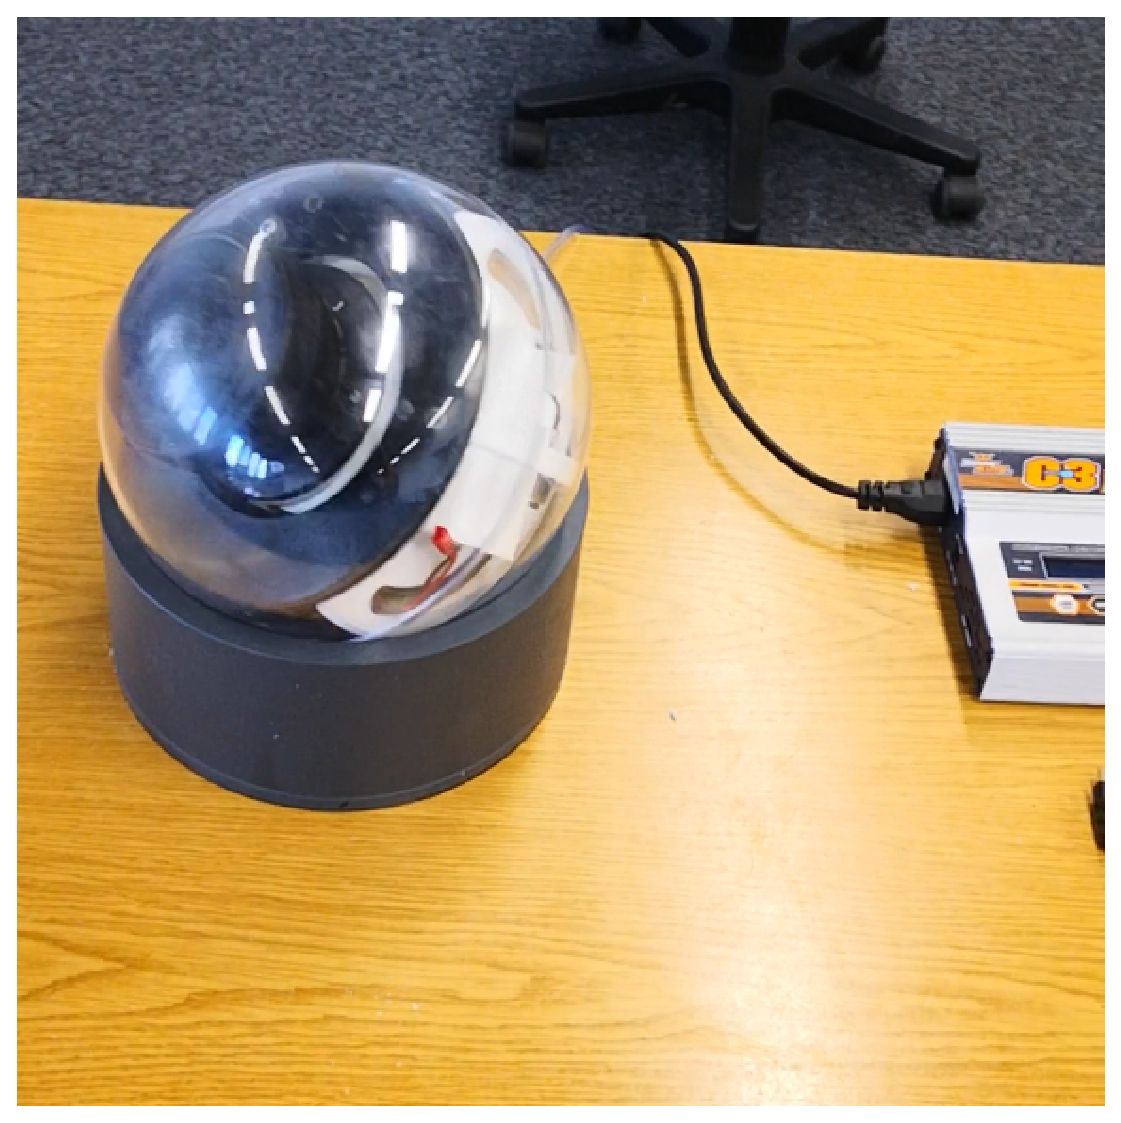
\includegraphics[width=0.33\textwidth]{./images/sphere-frame-1.eps}\hfill
		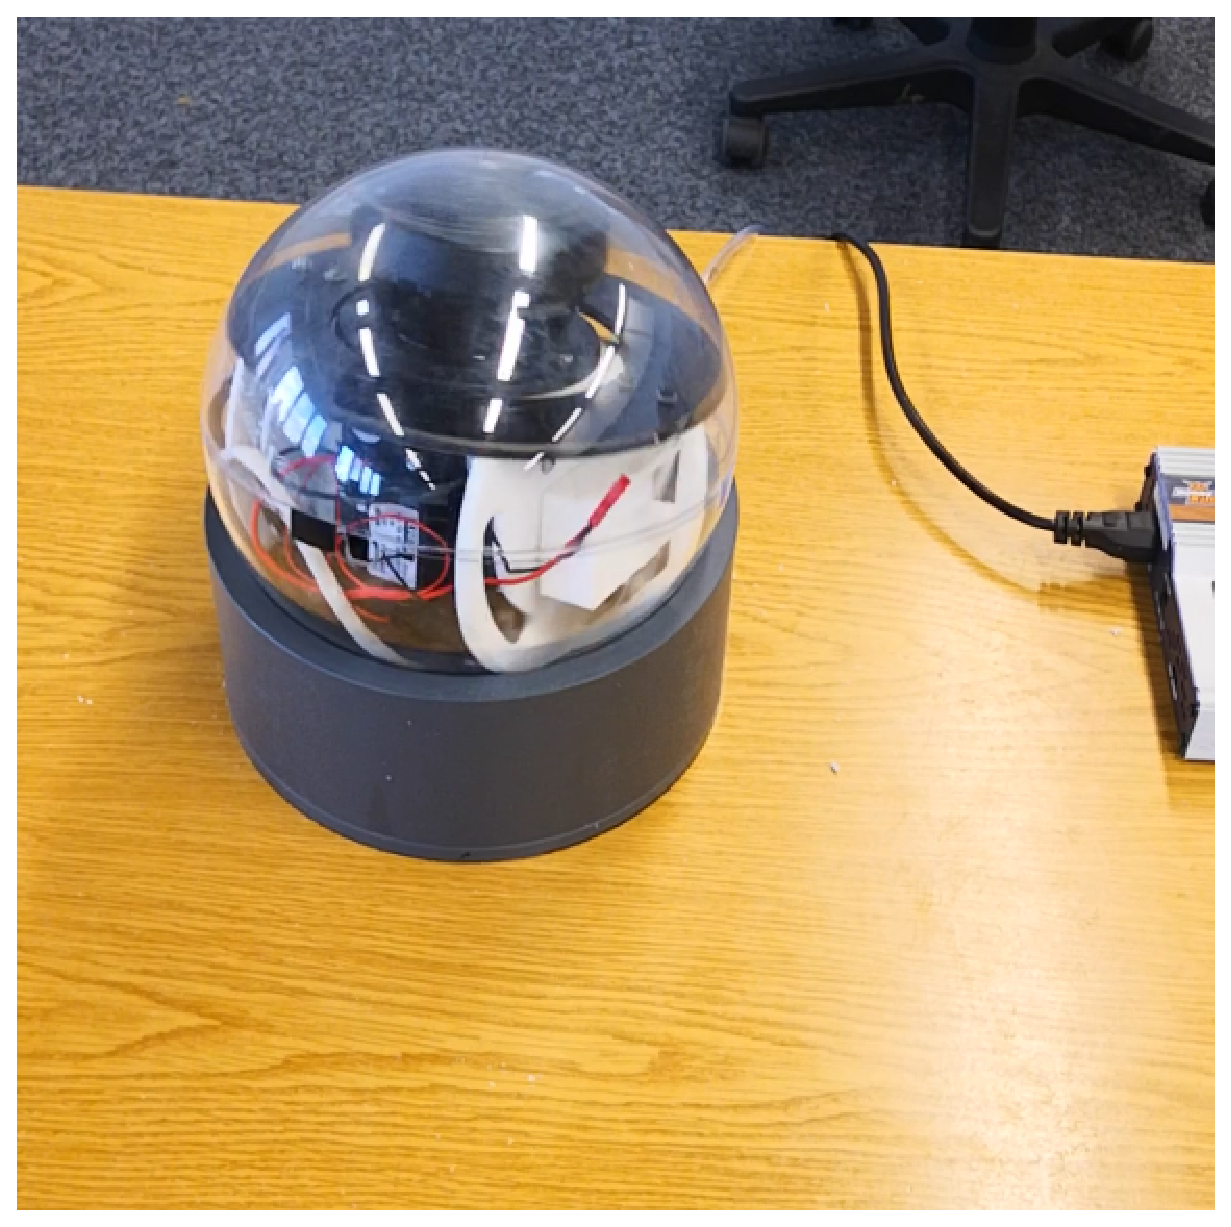
\includegraphics[width=0.33\textwidth]{./images/sphere-frame-2.eps}\hfill
		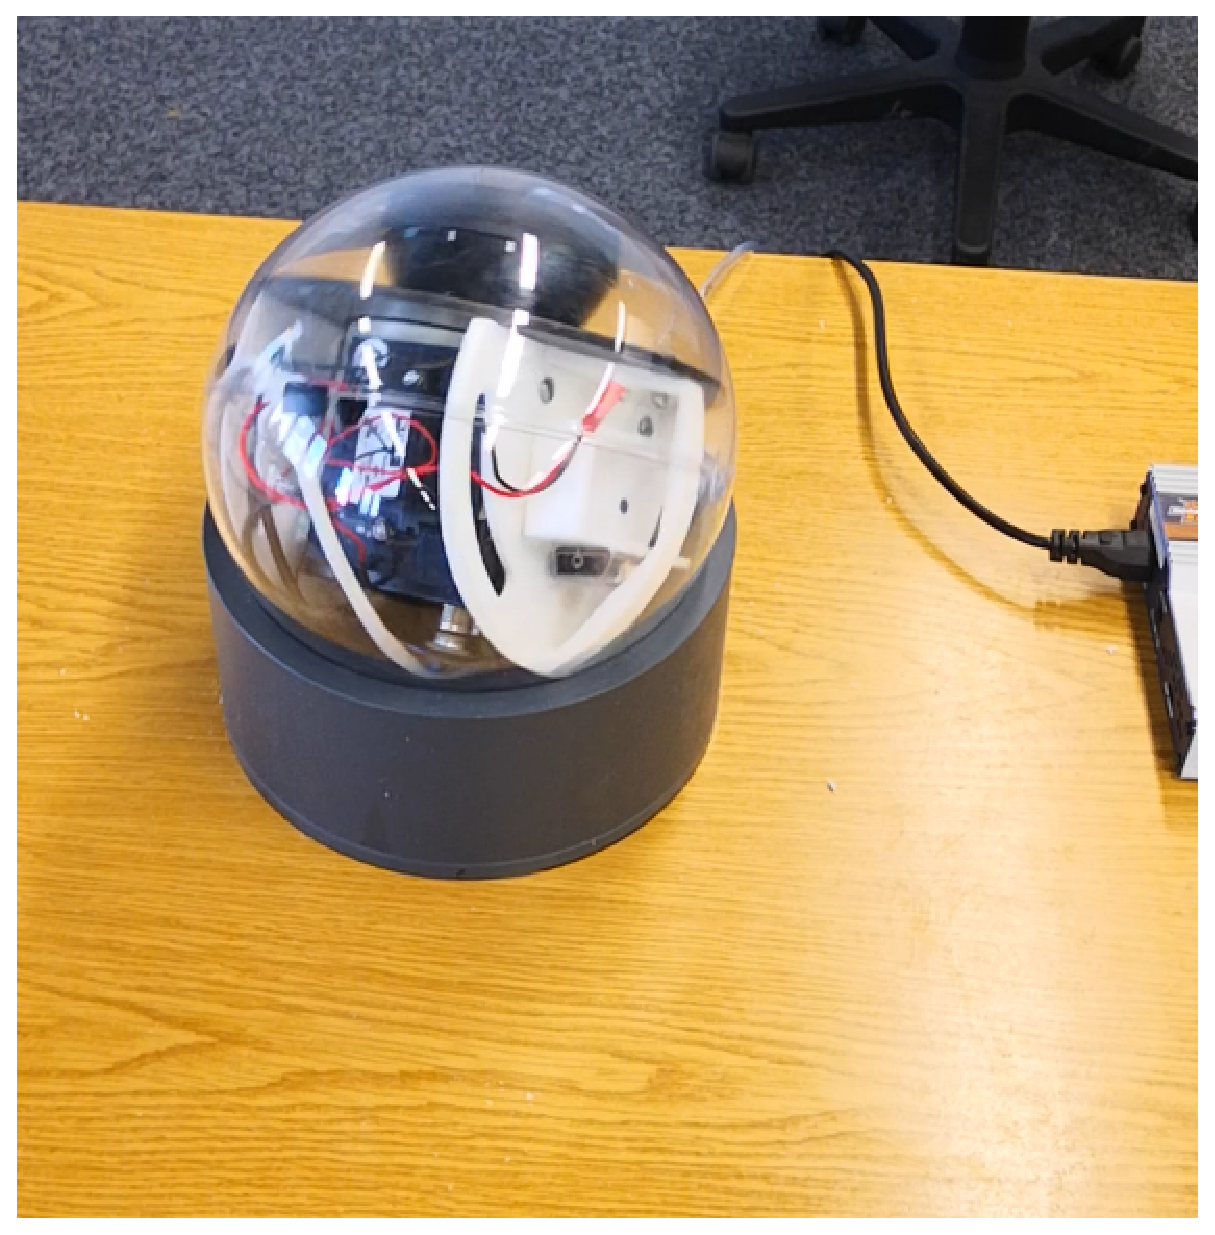
\includegraphics[width=0.33\textwidth]{./images/sphere-frame-3.eps}\hfill
	\end{minipage}\\
	\begin{minipage}[c]{0.5\textwidth}
		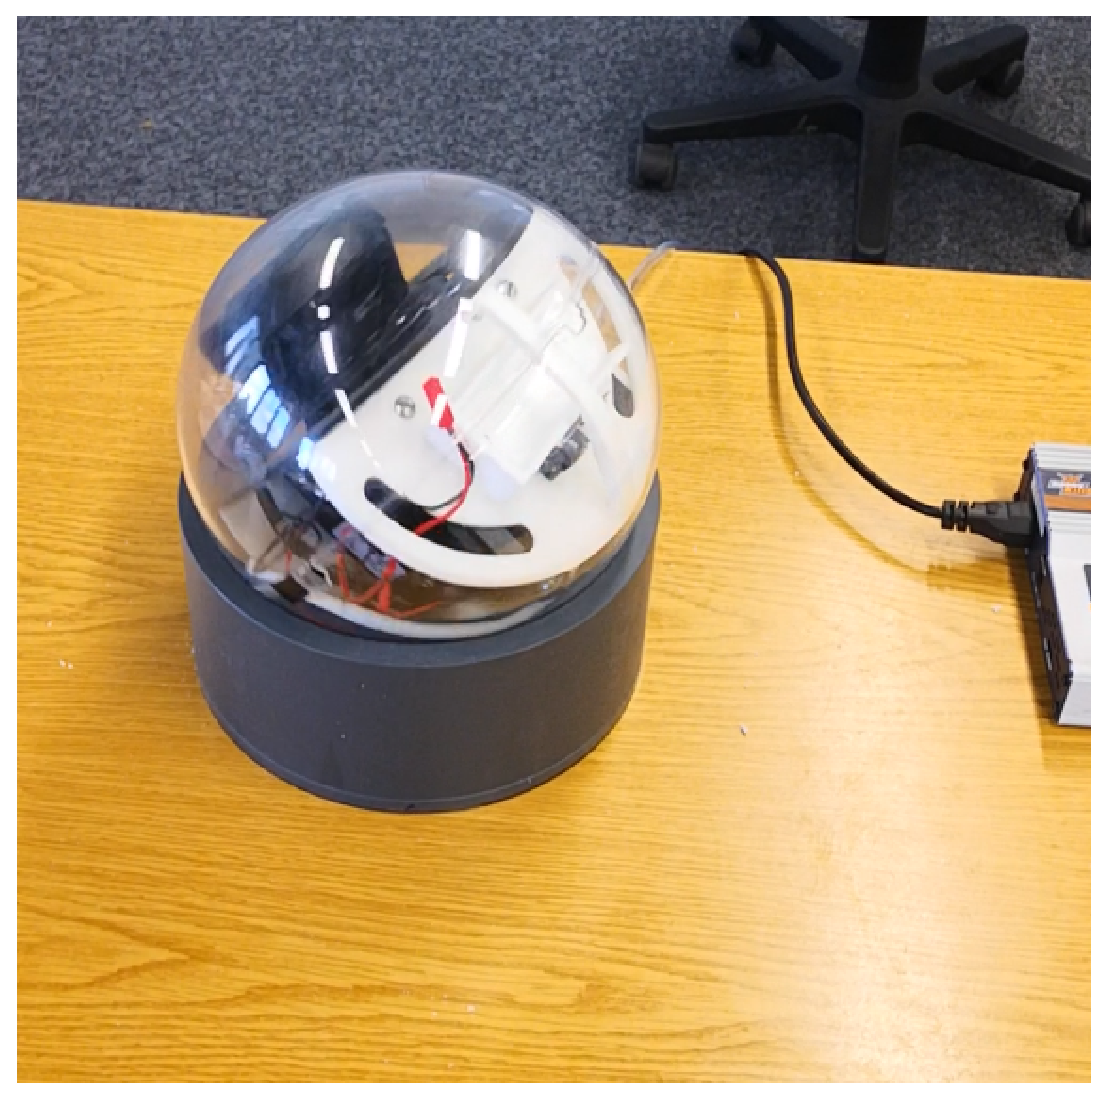
\includegraphics[width=0.33\textwidth]{./images/sphere-frame-4.eps}\hfill
		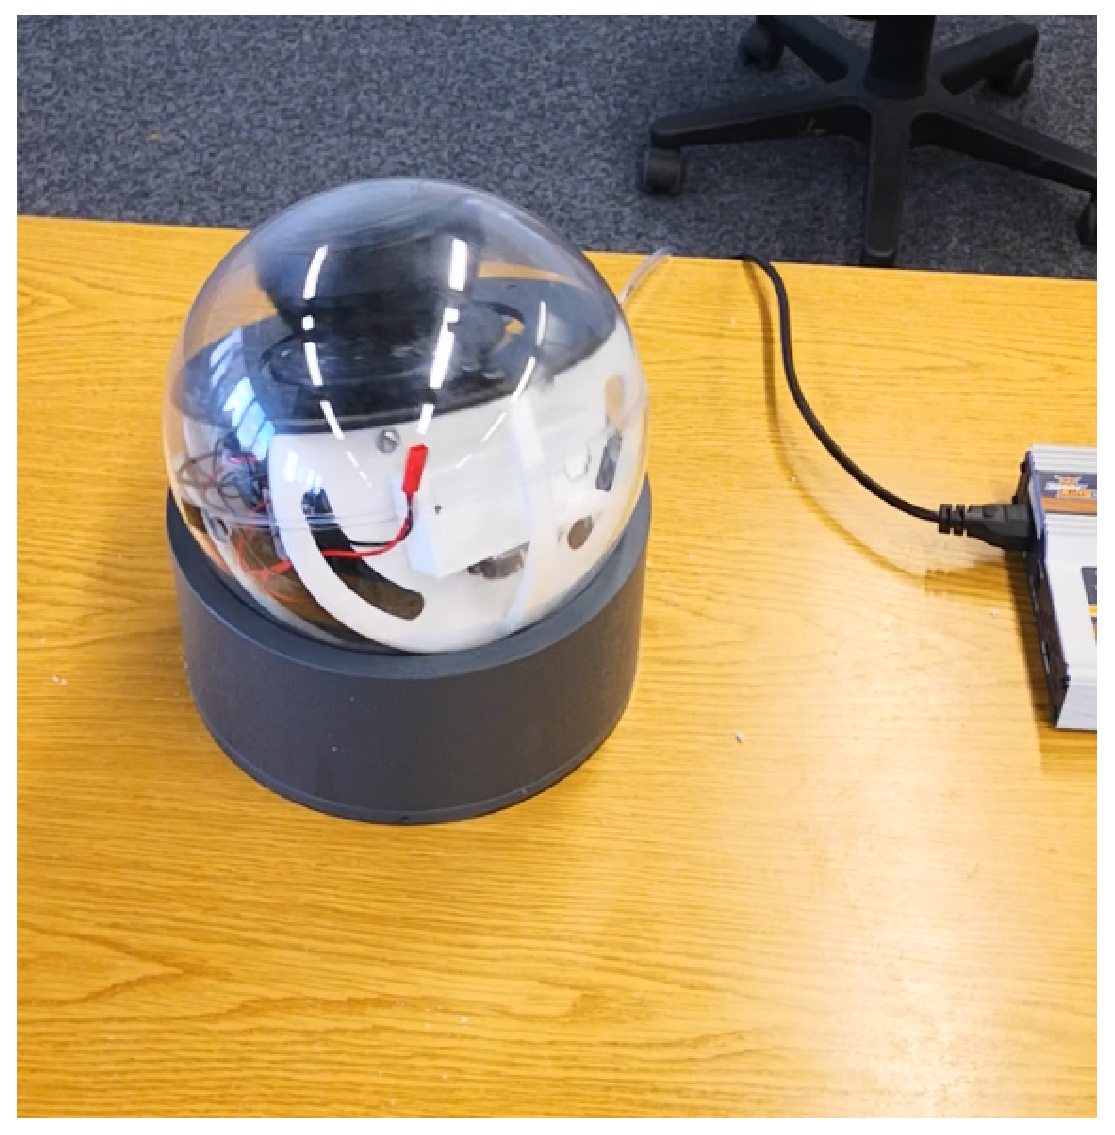
\includegraphics[width=0.33\textwidth]{./images/sphere-frame-5.eps}\hfill
		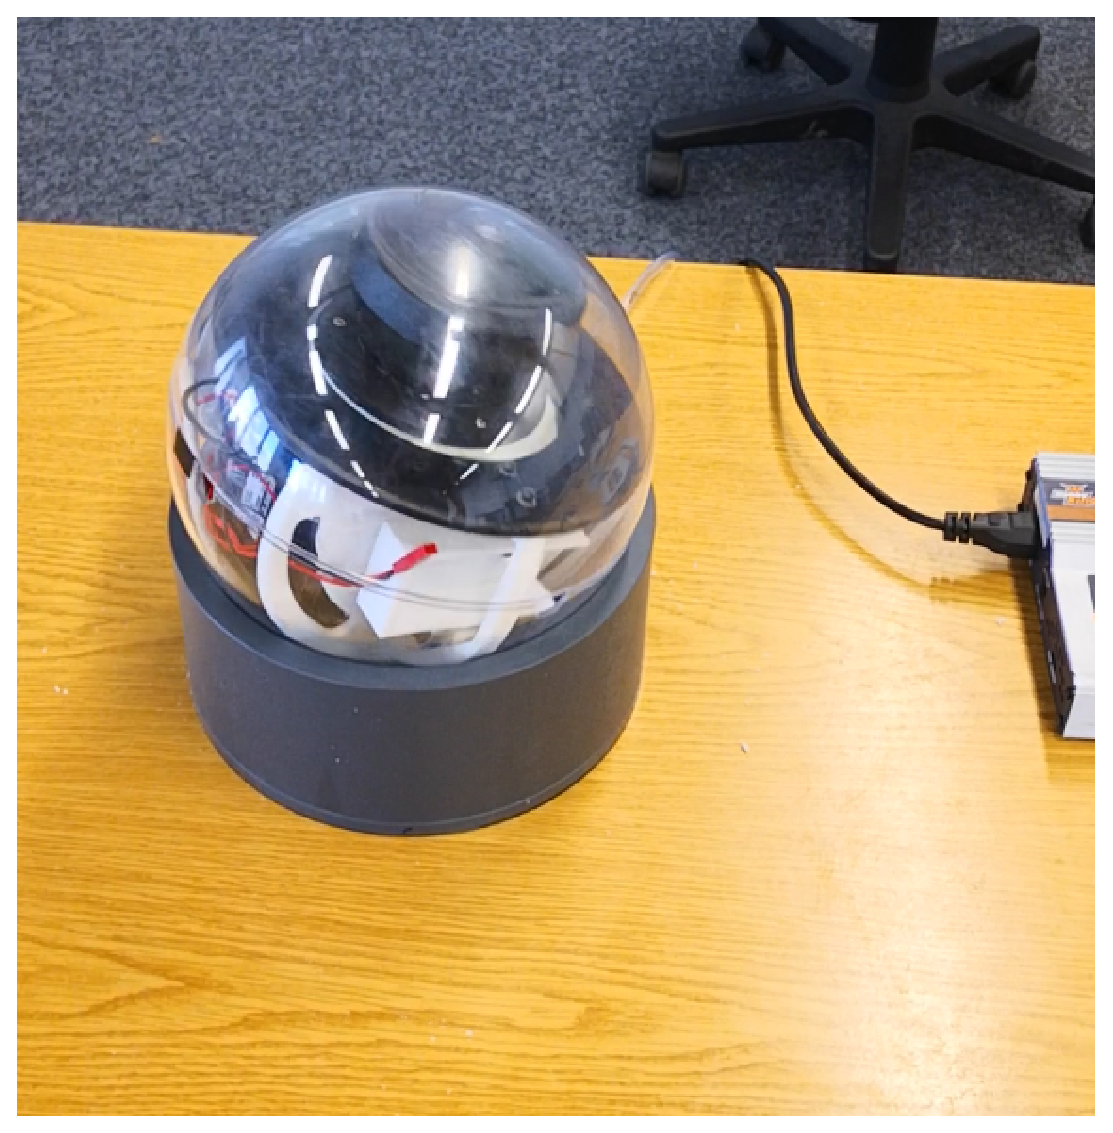
\includegraphics[width=0.33\textwidth]{./images/sphere-frame-6.eps}\hfill
	\end{minipage}\\
	\caption{Data acquisition using floating sphere. We show a sequence of orientations the sphere assumes.}
	\label{fig:float-sat-sphere}
\end{figure}

\subsection{RADLER}

The second dataset is recorded using the RADLER system as described in~\cite{Borrmann2020-RADLER}.
While not a spherical robot, this system shows many similarities with respect to its motion with a spherical robot.
The system was manually steered along a squared set of hallways that loop back to the initial starting point inside the old mathematics building at the University of Würzburg (denoted ``The Circle'' in~\cite{Borrmann2020-RADLER}).

Figure~\ref{fig:radler-mathe} shows the system setup as well as the resulting point cloud.
We see that with continuing measurement time the drift increases and the hallways are senses multiple times with a clear offset to each other. 

\begin{figure*}
	\centering
	\begin{minipage}[c]{\textwidth}
		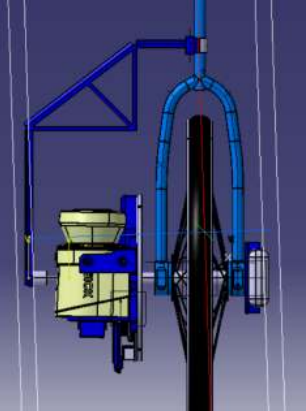
\includegraphics[width=0.2925\textwidth]{./images/radler_setup}\hfill
		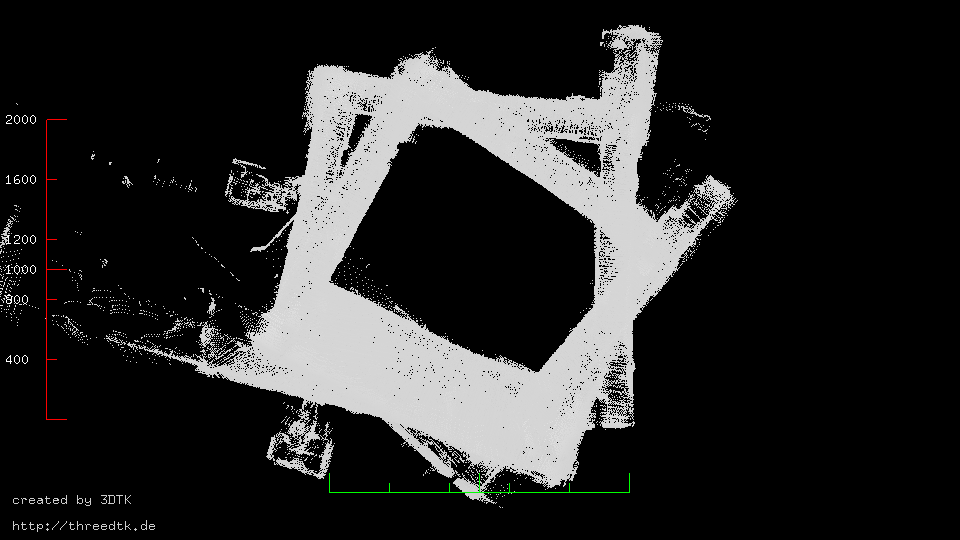
\includegraphics[width=0.7\textwidth]{./images/mathe_top_view}
	\end{minipage}
	\caption{Data acquisition using the RADLER system. Left: System setup (courtesy of Borrmann~\cite{Borrmann2020-RADLER}). Right: Unprocessed resulting point cloud.}
	\label{fig:radler-mathe}
\end{figure*}

\subsection{Descend Sphere REMOVE THIS SECTION}

This was recorded using a LIVOX-Mid 100 laser scanner mounted inside a transparent shell. 
The robot contained three Phidget 3/3/3 Spatial IMUs and was attached to a \SI{50}{\meter} tether cable that was rolled on a spool which in turn was connected to a angular encoder. 
From these sensors we obtained orientation information as well as height information. 
The setup was then brought into a high indoor building (\href{https://www.sfs-w.de/feuerwehrschule/virtueller-rundgang.html}{Firefighter School in Würzburg}) where the system was manually descended from a balcony scanning the building interior.
The robot covered a distance of approximately \SI{22}{\meter} in about \SI{402}{\second}.
Additionally the building was scanned using a terrestrial laser scanner to provide a reference.
The measurements were then rigidly corrected before applying our plane based correction. 
Figure~\ref{fig:experimental-setup} shows the acquired 3D point clouds and the experimental setup. 

\begin{figure}
	\centering
	\begin{minipage}[c]{0.25\textwidth}
		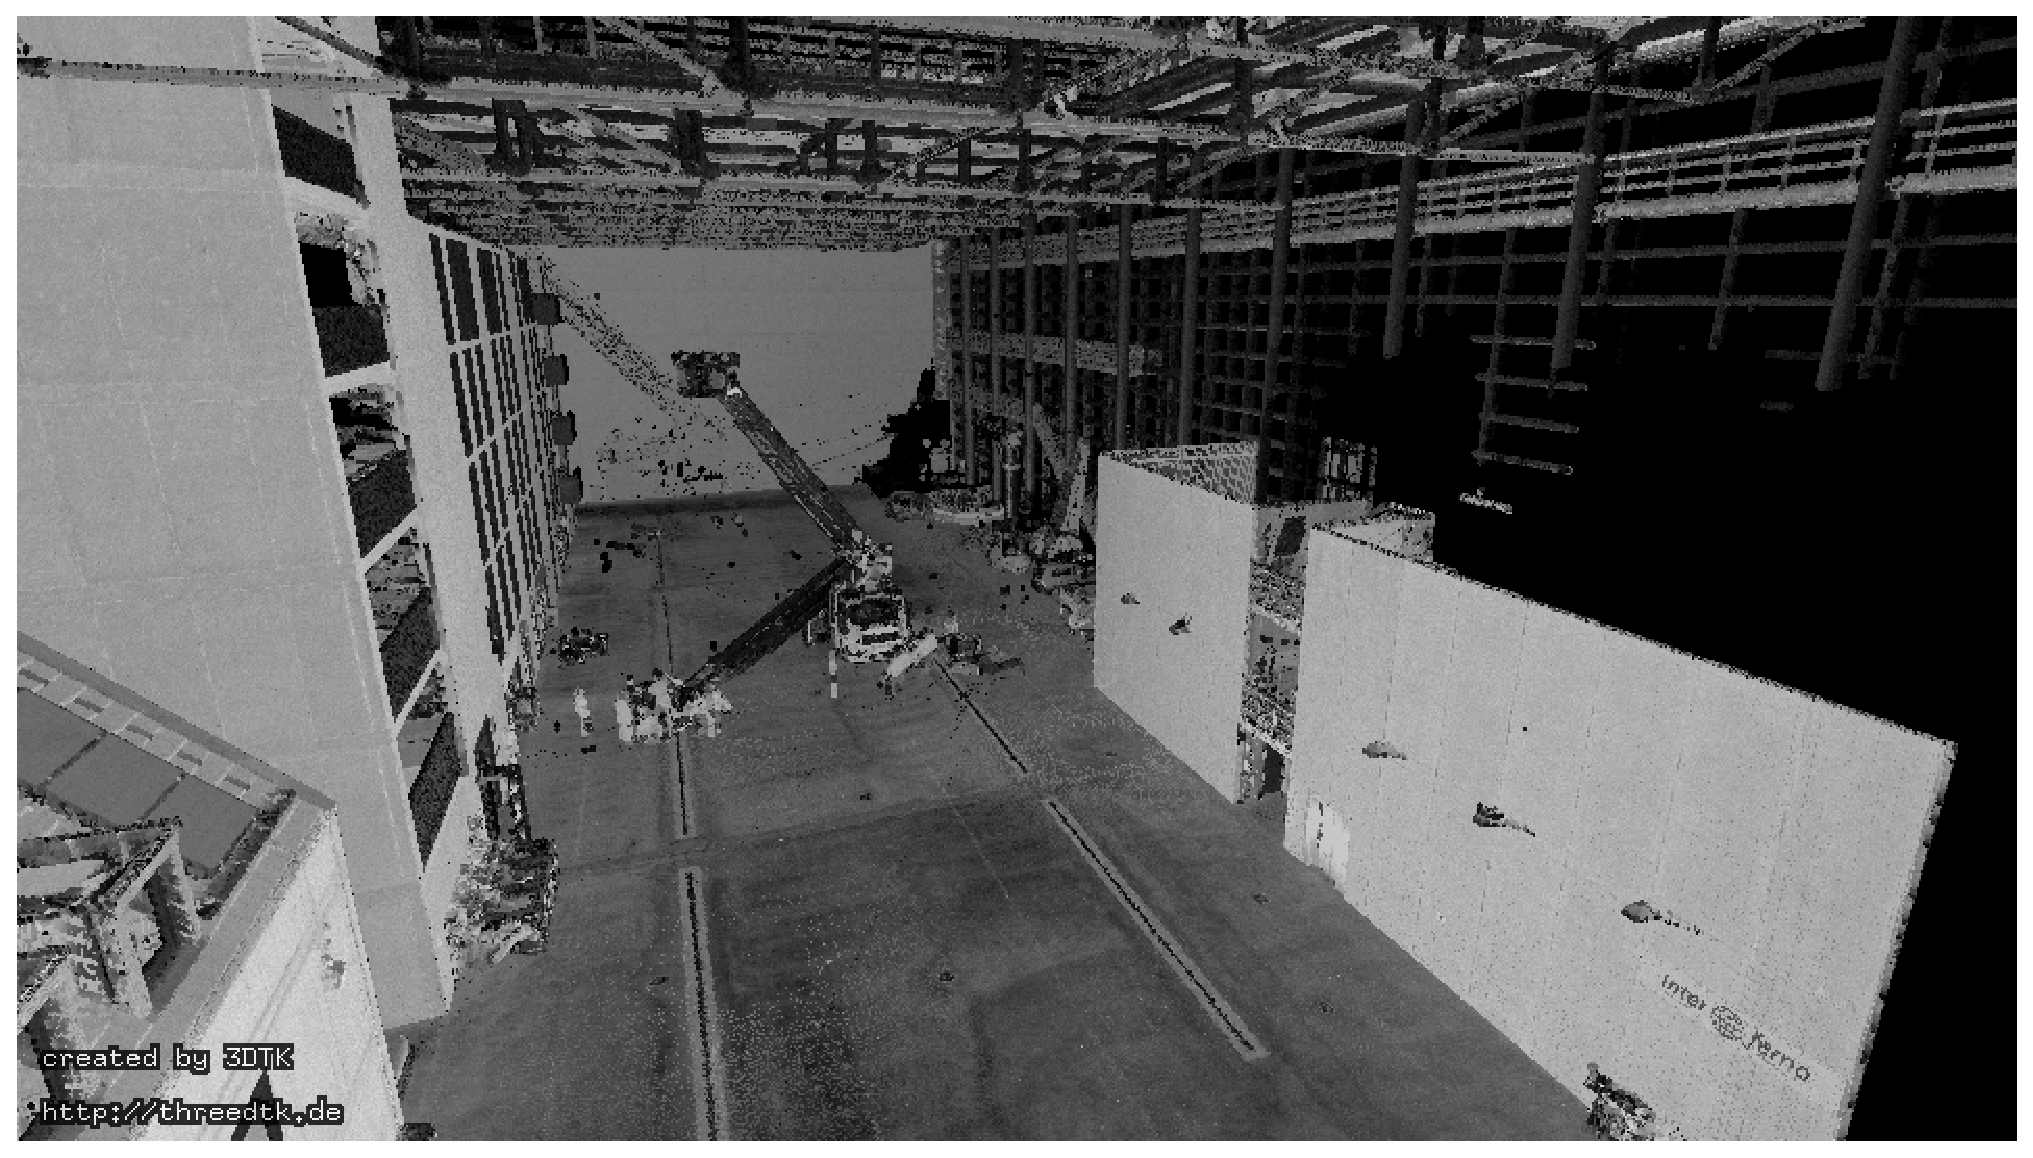
\includegraphics[width=\textwidth]{images/scan-riegl-fire}\\
		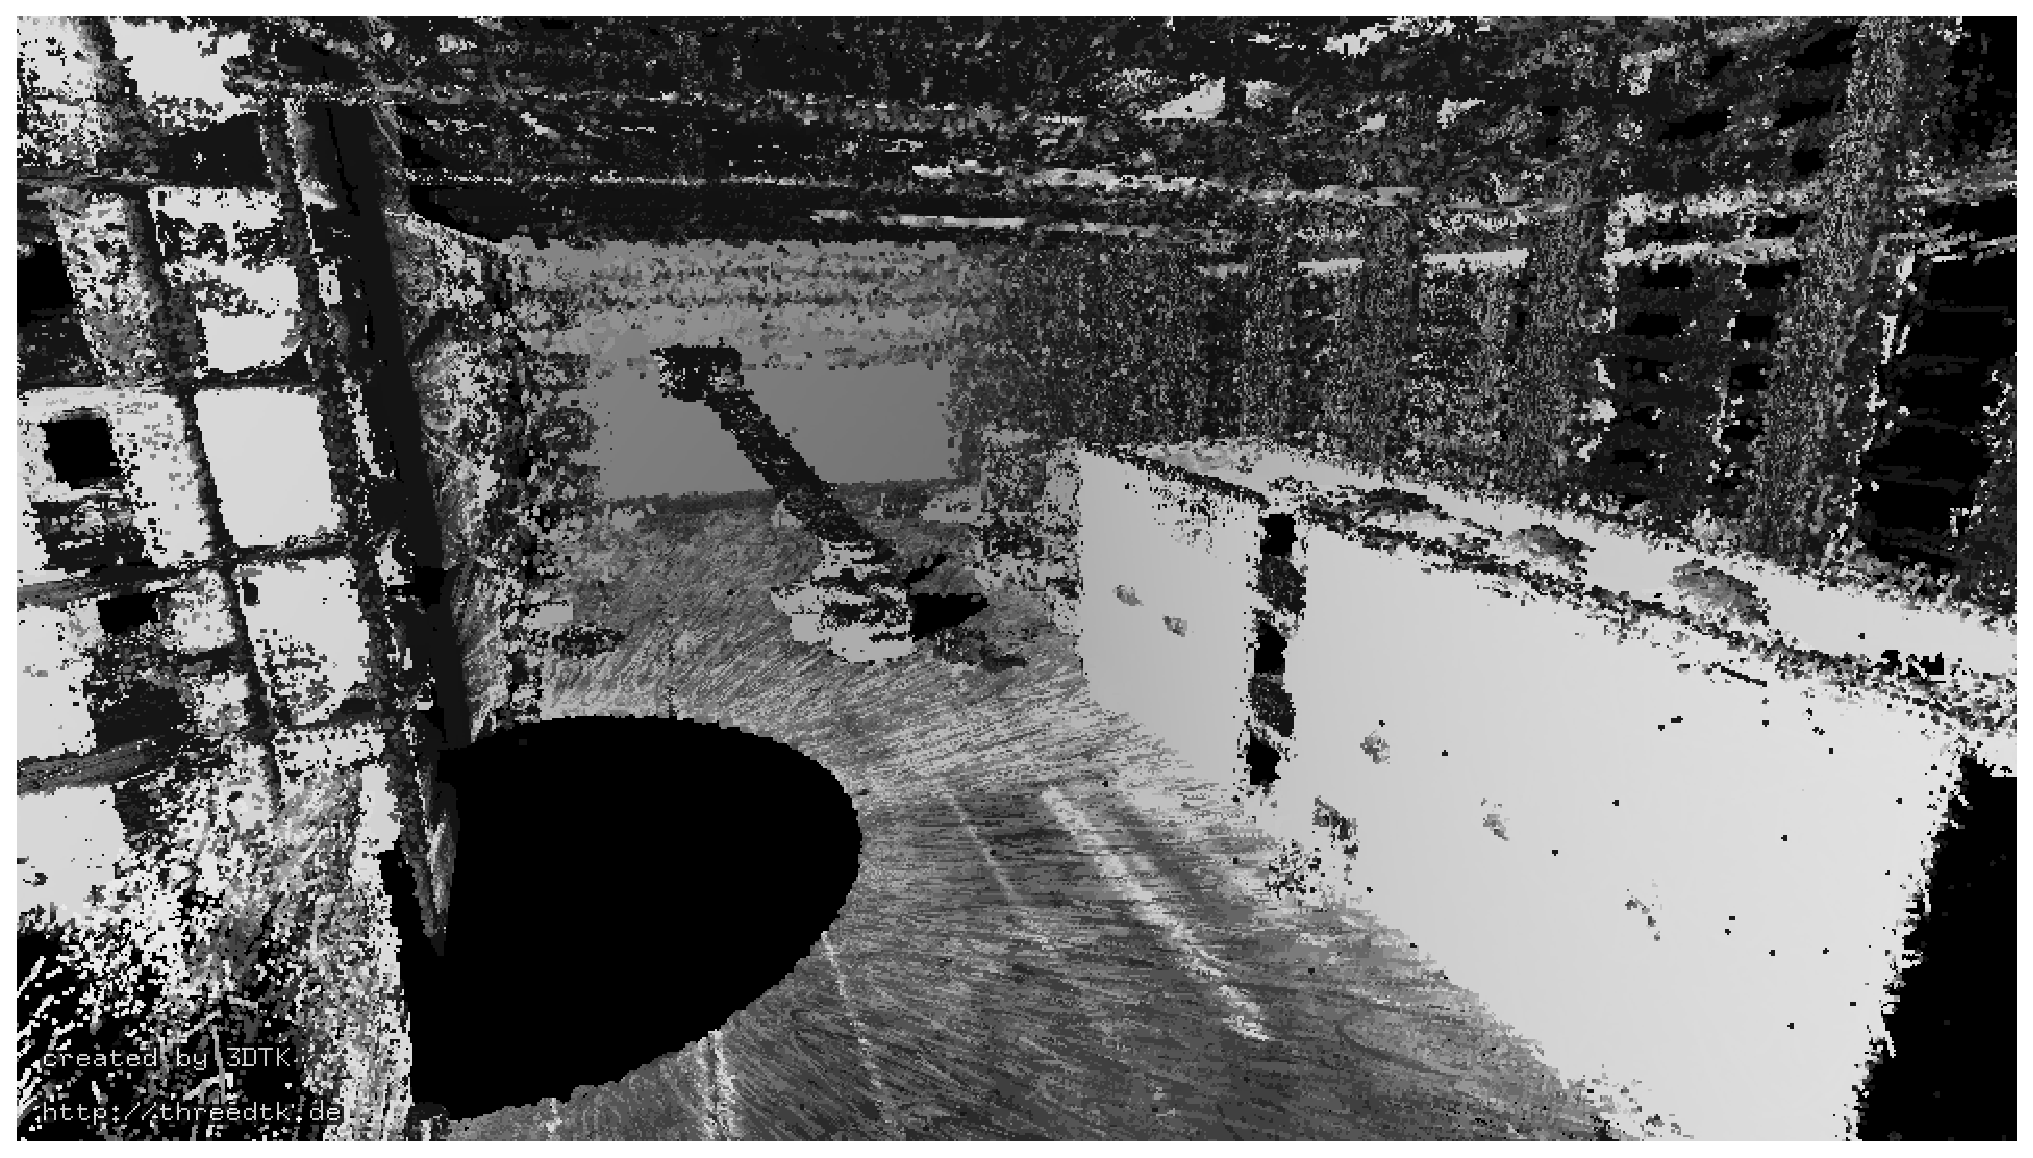
\includegraphics[width=\textwidth]{images/scan-sphere-fire}
  	\end{minipage}\hfill
  	\begin{minipage}[c]{0.2075\textwidth}
  		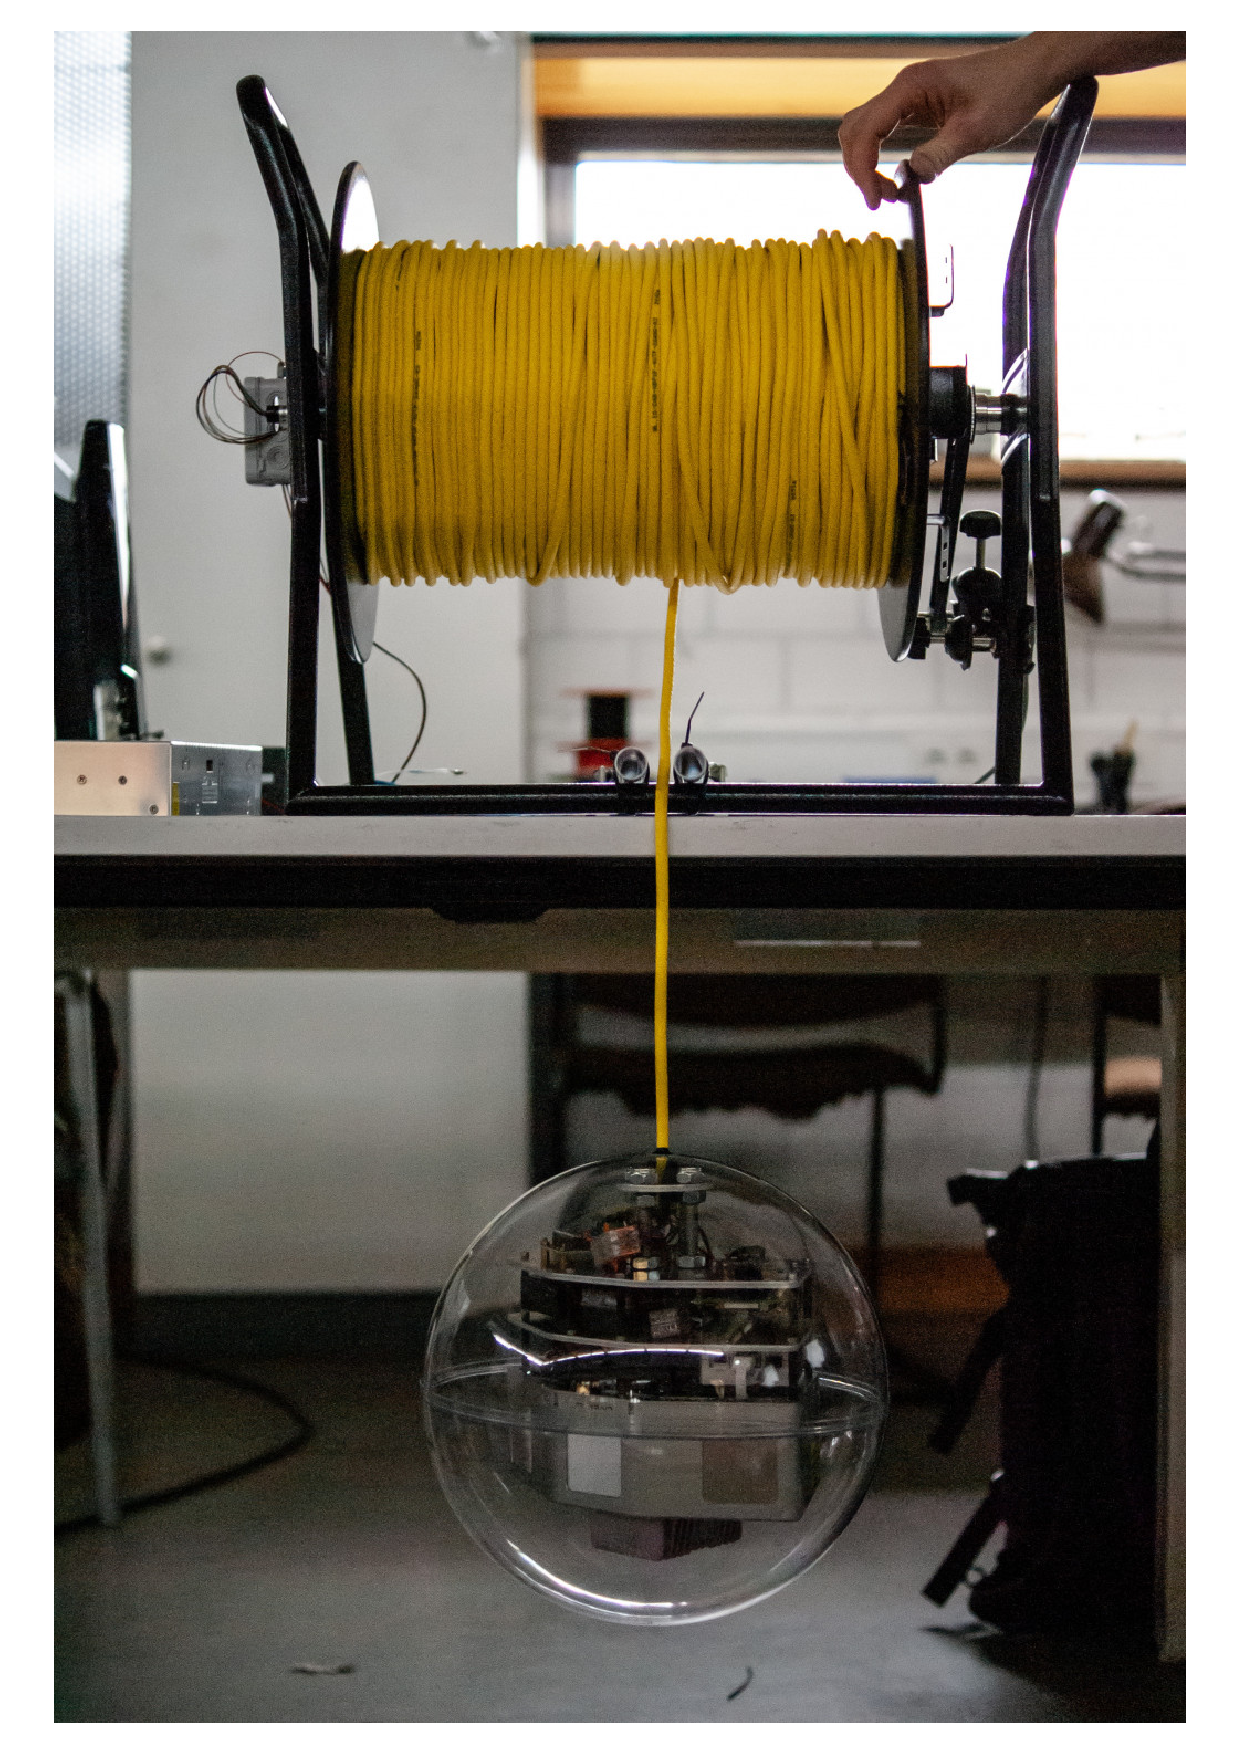
\includegraphics[width=\textwidth]{./images/lidarsetup}
  	\end{minipage}
	\caption{Reference 3D point cloud acquired with a RIEGL 3D terrestrial laser scanner (top left). The 3D point cloud acquired by the test sphere after the rigid registration (bottom left) and a picture of the test setup (right).}
	\label{fig:experimental-setup}
\end{figure}




